%!TEX root = ../main.tex
%=========================================================

\section{Introduction}

\er{Suggested refactoring. I would start directly by explaining the Ethereum decentralized network supports multiple applications in addition to the mainnet used for the Ethereum blockchain. I would not attempt to keep the discussion general about P2P network, their capitalization etc. Rather:
\begin{itemize}
  \item Ethereum supports multiple applications. These applications vary in size. How their number is expected to grow in the future. Make the case for scalability
  \item Managing membership is crucial, what attacks we need to avoid (partitions, eclipse, etc.)
  \item Bootstrap nodes are not desirable and why (give concrete examples of decentralized networks that actually use them as this is unclear in the current text, and it seemed to me that Ethereum used a flooding based discovery that is already decentralized) -- keep this only if there are examples of decentralized networks that do use them we can cite.
  \item Explain discv4 and how it addresses robustness concerns but not scalability
  \item Traditional way to address scalability is to use a DHT but this leads to robustness problems
  \item Explain the contribution.
\end{itemize}
Note that there is some text in the overview that can be reused. (Two first paragraphs of section 5)
}

In recent years, peer-to-peer (P2P) networks experienced a rapid growth. They are widely used to support supply chains, collective file storage, cryptocurrencies, decentralized finance and non-fungible tokens. The market capitalization of the P2P networks supporting uniquely cryptocurrencies already exceeds 1.8 Trillion USD. 

%Ethereum~\cite{buterin2013ethereum}  is the largest permission-less (\ie open membership), open-source blockchain supporting Turing-complete scripting via smart contracts. 


%Services require dedicated \emph{sub-networks}, each consisting of only the peers participating in a particular application. A \emph{sub-network} enables the exchange of application-specific data, such as transactions and blocks, only between the interested peers. 
Before a P2P network can be formed, its peers must first discover each other. The process of finding peers is crucial for the security of the entire system and is considered a first-class problem in blockchain networking~\cite{dotan2021survey}. Operations of even largest networks can be effectively disrupted when its nodes cannot find each other. Worse even, a node using an unreliable peer discovery protocol may be fed a list of malicious nodes and become completely detached from the network. In the context of blockchains and cryptocurrency, service discovery eclipse attacks can lead to double-spend attacks, stubborn mining and endanger the security of financial assets. \er{references?}

In practice, the vast majority of currently-operating P2P network use bootstrap nodes to initiate a peer discovery process. Those nodes are usually maintained by foundations taking care of the ecosystem (\eg Ethereum Foundation, Bitcoin Foundation) and hardcoded in the client software. Bootstrap nodes return a pseudo-random sample of the current network participants, enable newcomers to join the P2P network and discover more peers. 

The bootstrap nodes, while practical, are also problematic. They are a critical trusted party of the ecosystem, require significant amounts of money to maintain and must be secured to prevent a vast range malicious behaviours. While the largest P2P networks such a Bitcoin, BitTorrent or Ethereum have the user trust and funds to ensure a reliable network of bootstrap nodes, such solution in highly unsuitable for developing P2P systems.

As a result, large, well-established P2P systems are often used as a replacement of centralized bootstrap nodes and enable the peer discovery process for a whole plethora of smaller networks. The Ethereum network, primarily developed to support the Ethereum blockchain, is also used by third-party, guest applications such as testnets (Ropsted, Rinkeby), alternative cryptocurrencies (Pirl, Musicoin), content delivery (Swarm) or messaging (Whisper). We refer to them as \emph{applications} or \emph{services}. In 2018, the Ethereum P2P network nodes operated a total of 4,076 different applications (\Cref{fig:ecosystem}), and this number is expected to grow in the future~\cite{kim2018measuring}. However, an application-specific newcomer that joins a host P2P network still needs a \emph{service discovery} protocol to find its application-specific peers. 

\begin{figure}
    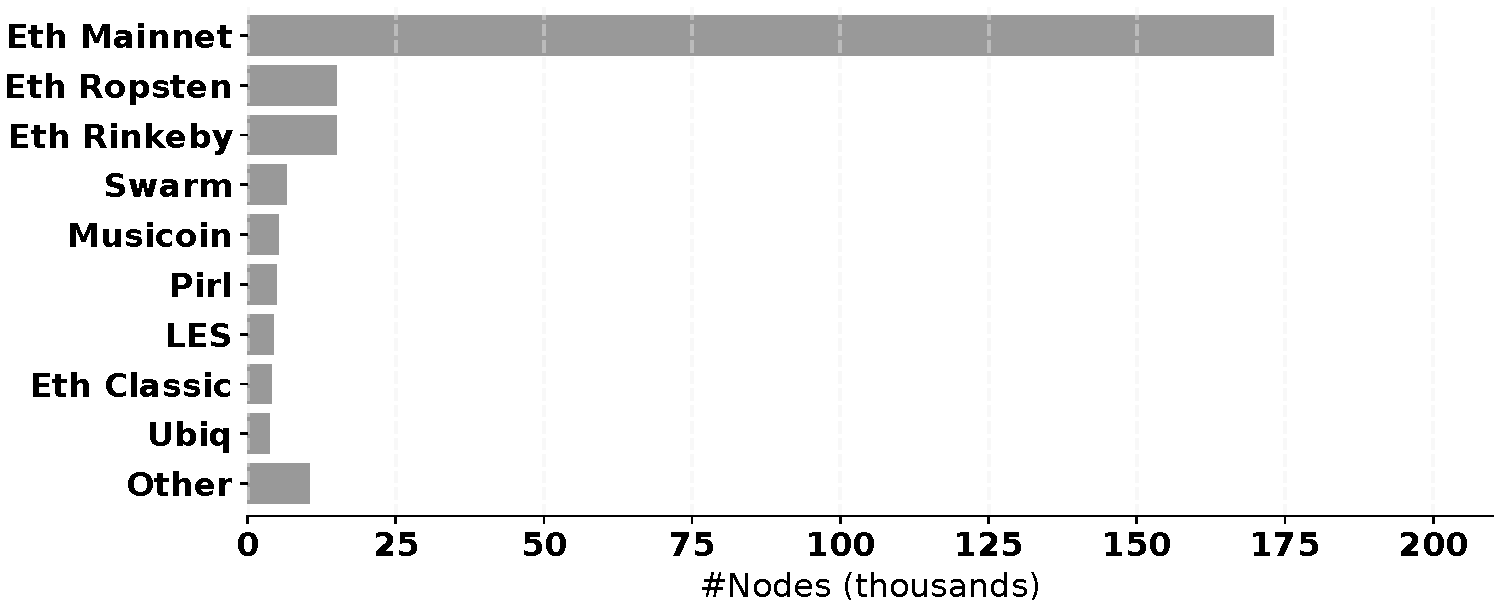
\includegraphics[width=1\linewidth]{img/ecosystem}
    \caption{Sub-networks in the Ethereum ecosystem.
    \protect\er{maybe give the date when the snapshot was taken. Also, ``Other'' should be ``Others''. We can also consider using a split x axis in order to avoid the very small lines for everything else than the mainnet. The figure is also not giving a sense of the long tail with networks of a few hundreds/thousands of nodes (our focus)}}
    \label{fig:ecosystem}
\end{figure}

%\michal{As Onur suggested, we should discuss more the advantages of having a large, common network to start with (rather than build a seperate one for each app). One point would be to argye that currently used bootstrap nodes are a critical point of the whole system. We can make them secure in big networks (with a lot of money). But that's difficult to ensure in small networks. Thus it's easier to go first to Ethereum and use our system for discovery.}

%\michal{Value of high quality nodes that you can't get easily. DHT is like wine (the older the better). Resilience. It's a barrier for smaller projects to set up their network and bootstrap nodes etc. Here, it's instant. Bittorrent DHT was is being used by different networks, because its already there and working well.}

%\michal{Does the walk in discv4 exposes nodes to some additional targeted attacks? Once you're discovered (by asking others) you can be targeted.}

\para{State-of-the-art} Ethereum currently uses a decentralized, general-purpose Distributed Hash Table called 'discv4' for the purpose of \textit{service discovery}, \er{this contradicts the earlier text that said Ethereum used bootstrap nodes maintained by a foundation} enabling any node to discover \textit{a random sample} of all available peers. A node first \textit{(i)} joins the (application-agnostic) discv4 network, \textit{(ii)} discovers application-specific peers and \textit{(iii)} joins a sub-network by connecting to the discovered peers as shown in \Cref{fig:subnetwork}. The discv4 protocol is loosely based \er{what does loosely based mean?} on Kademlia~\cite{maymounkov2002kademlia} – a well-established Distributed Hash Table (DHT) approach. Discv4 uses a simple, brute-force discovery mechanism involving random walks in the DHT containing peers from all ranges of applications. Throughout this paper, we refer to this approach as DISCV4RANDOM. Each random walk encounters random peers which are then supplied to the application. The application determines whether the supplied peers support the desired application through dedicated handshake messages. The process continues until a desired number of connection slots are filled. 

With the built-in randomness of DISCV4RANDOM, Ethereum is relatively secure against denial-of-service and eclipse attacks. Each node queries an unpredictable set of peers regardless of its application. As a result, an attacker cannot easily stop the process or strategically place its Sybil identities.
However, the overall process is highly inefficient and generates significant message overhead. This is especially visible for unpopular applications with a small number of peers.  For instance, assuming an application with 10 nodes in a network of 5,000 nodes, a newly-joined node needs to perform on average 500 handshakes to find a single peer. \er{can we have actual numbers from the current network?} As more applications join the DHT, the inefficiency of the brute-force DISCV4RANDOM discovery process becomes a bottleneck. While other alternative solutions for peer sampling have been proposed, they are impractical~\hl{[]}, based on unrealistic assumptions~\hl{[]} or insecure and rarely used in real-life. We provide an extensive analysis and comparison of these systems in \Cref{sec:related}.

%The randomness in the sampling of peers in both the DHT-level connections by Kademlia and application-level connections by Discv4 provides (a best-effort) Byzantine resilience in a permission-less network where financially-motivated attacks targeting individual applications are common. \er{I would not go as far as to write that it is Byzantine-resilient. It is a mitigation, but it has limits.} \er{is Kademlia used for something else than the random walk?}

%In addition to security, another major challenge facing service discovery is the \textit{scalability}: although random peer selection provides an acceptable-level of security against eclipsing attacks, the current discovery process is rather slow in finding peers for even moderately popular applications. \er{Does not strike me that discv4 is really subject to security problems, in the very worst case you could ask all peers in the network and would be guaranteed to get the $n$ ones you are looking for following topic $t$.} 
%\dk{If large parts of the network are eclipsed, all nodes offering a certain topic/service might be unreachable. Eclipse attacks can prevent nodes from being able to ask all peers.}

%\dk{Could provide a simple model showing this. I have done a basic calculation, which I will link in the PR.}
%\dk{Waku v2\footnote{\url{https://wakunetwork.com}} is such an application. We discussed the shortcomings of random-walk discovery and are planning to implement more efficient means. You could list Waku as a motivation/example of an application that wants more efficient discovery means like the topic table this paper proposes.}

\para{Our Contribution} In this work, we propose \sysname - a new \textit{service discovery layer} which enables secure, efficient and robust discovery of application-specific peers in the Ethereum network.
Different from DISCV4RANDOM, our \sysname allows nodes (\ie advertisers) to associate themselves with a set of \emph{topics} (\eg application IDs), and advertise this association in the network. \er{as a reader I would think ``they are reinventing the DHT''. Why don't we simply detail that DHTs are the go-to solution for scalable membership management in the absence of faults, and explain why we need to do differently because of these?}

The information is collectively stored by network participants (\ie registrars) without relying on a single trusted party at any point. Any node can then query the network for a topic to obtain a list of application-specific peers and directly connect to them without disturbing members of other sub-networks and applications. 

We build \sysname on top of the existing Kademlia-inspired DHT to propagate application-specific advertisements to randomly-sampled nodes to make deliberate attacks on the network costly to mount and persist. Our design encourages diversity of advertisements stored at each registrar making the system resistant to network dynamics and partitions. At the same time, \sysname provides efficient peer discovery operations terminating within a certain maximum number of steps (logarithmic in the network size) for all the topics regardless of their popularity. 

\felix{Is this claim really true? Log complexity search for all topics?} \er{this is the classical claim for a DHT lookup (and is guaranteed by the overlay structure). However, this is more complex to prove in the presence of faults and polluters.}

An open system allowing any node to place advertisement requires an admission protocol. \er{at this stage this is still unclear that we allow advertisements on any node, and not only on nodes that have a specific position in a key space. The paragraph might be already quite specific to the solution and therefore easy to misinterpret.} Each registrar, having limited storage capacity, must decide which ads to accept and when to expire them. Doing this correctly is crucial for system security and robustness in a highly dynamic environment. \sysname implements a lightweight admission mechanism which limits the resource usage on all nodes (registrars and advertisers), ensures fairness across topics, and prevents many common opportunities for malicious behaviour.

\para{Contributions} We make the following contributions:
\begin{itemize}
    \item In \Cref{sec:placement}, we design a DHT-based data placement system that distributes service advertisements in the network. The protocol combines pseudo-random data placement for security \er{not sure what is meant by that?} with deterministic operations for efficiency. We present a lookup operation that finds a subset of ads placed in the system within a bounded amount of time. Our procedure ensures diversity of data sources and is resistant against manipulation by malicious registrars. 
    \item In \Cref{sec:registration} we design a lightweight admission protocol allowing advertisers to place ads after waiting for a specified amount of time. %\er{I would mention the problem and not only the solution here (make continuous registration of fake/malicious entries more complicated and limit their impact)}\mk{We've now added motivation for that in the paragraph just before the contributions} 
    \sysname guarantees that advertisers cannot place more advertisement at a specific registrar by deviating from the protocol %\er{is this completely true? I understood they could place more, but not many times more?}\mk{now it is. we ensure that with the lowe bound mechanism}
    and does not create any intermediary state at nodes holding the advertisements.
    \felix{This claim, needs some serious rewording. Only us authors understand that 'intermediary state' here means 'state of potential registrations'.}
    
    \item In \Cref{sec:waitingTime}, we design a function that calculates a waiting time after which advertisement can be placed on nodes holding advertisements. The function limits the amount of resources used by each node, promotes ads diversity stored within nodes, and protects against a vast range of malicious behaviours. 
\end{itemize}

Our evaluation shows...


\begin{figure}
    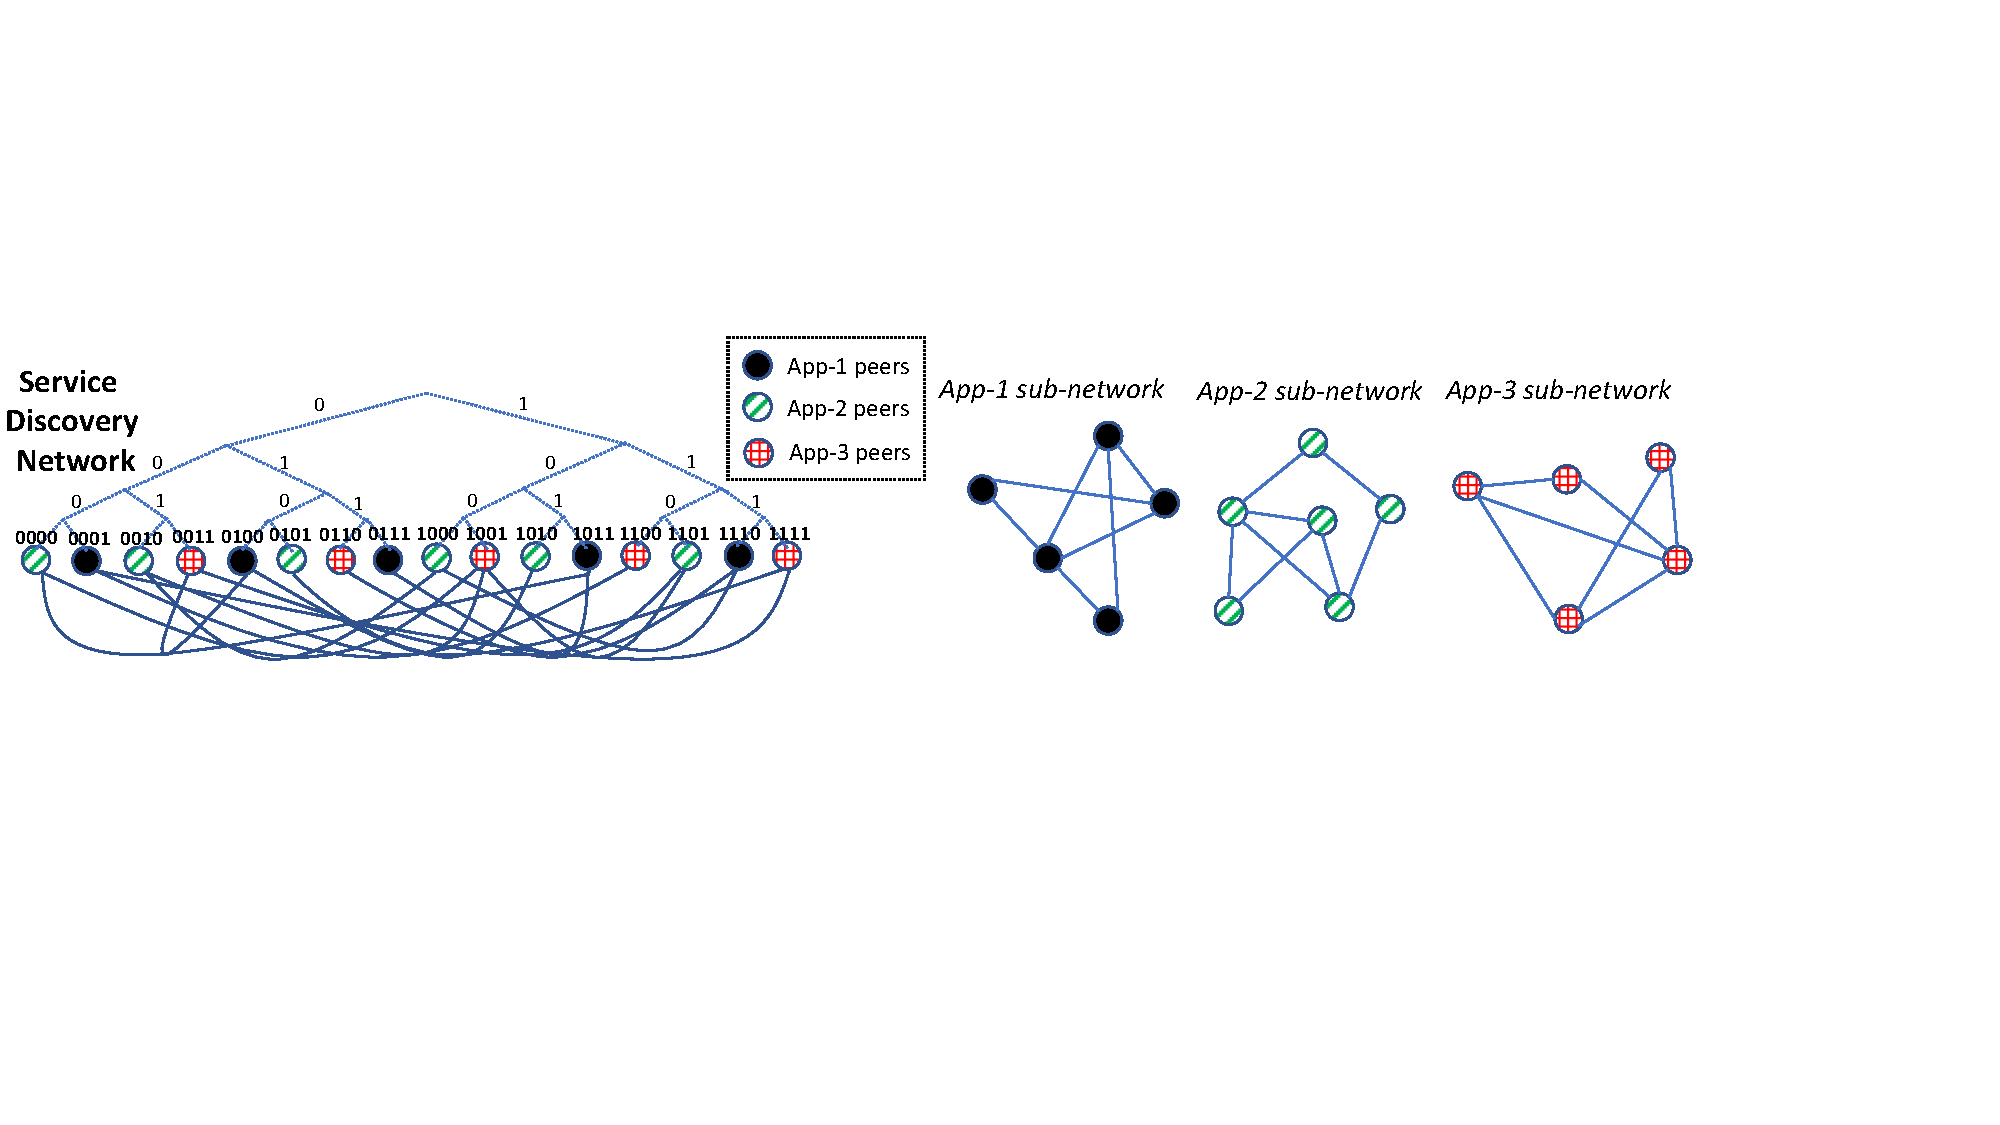
\includegraphics[width=1\linewidth]{img/subnetwork}
    \caption{Formation of application-specific sub-networks using a universal service discovery network.}
    \label{fig:subnetwork}
\end{figure}



%Rather than each application building its own, dedicated peer discovery protocol where only the peers of individual applications participate, 


%The discovery process continues until an application-specific number of connections are successfully established with live peers. 
% \er{to discuss: ``service discovery'' could be understood as locating the single server in charge of a service--this term is often used in SOA. In the P2P world, I have seen the term ``membership management'' used as well to denote the discovery of a random set of peers from a group (seminal paper is SCAMP~\cite{ganesh2003peer}). We should preferably use the term used in the ETH community but we can give the precision in the RW section (I can do it).} % Onur: I think I addressed this now.





%An important feature of a large, general-purpose service discovery network is its ability to withstand security attacks: launching a successful attack against a protocol run by many applications' peers requires more resources than launching one against an application-specific discovery protocol with (at least initially) small number of participants. Security of the discovery protocol is especially crucial in the presence of financially-motivated attacks targeting cryptocurrency-based applications; a common one is a combination of \textit{eclipsing} and \textit{Sybil} attacks, whose purpose is to fill up a peer's connection slots to discovered peers with Sybils, which then collectively feed the peer incorrect information, \eg incorrect state of the application's blockchain, as part of a larger attack such as double-spending, stubborn mining, and so on. 

%For instance, a blockchain node that cannot find honest peers or is fully eclipsed by malicious peers might accept an incorrect state of the blockchain. These application-level attacks use as a precursor the more basic, targeted attacks such as eclipsing where an attacker aims to fill up a peer's application-level connections with its Sybils - afterwards, an application can be fed with any custom data as part of an attack such as double-spending, stubborn mining, \etc. 
%\er{This is a bit light in terms of motivation imo. We need to make it very clear that our primary target is to resist eclipse attacks, so I would give more arguments about what malicious nodes can do in our model here (without detailing the said model yet)}

%The Ethereum network is based on Kademlia\cite{maymounkov2002kademlia} – a well-established Distributed Hash Table (DHT) implementation. 
%Unlike the earlier DHT systems, Kademlia follows a flexible peer selection process that allows random sampling of peers from each distance-specific interval along the circle (where identifiers are arranged). 
%Each node establishes \textit{DHT-level network connections} with a fixed number of sampled peers from each distance and also adds those peers to the corresponding (distance-specific) entry in its local routing table.
